\documentclass[sigconf, authordraft]{acmart}

\usepackage{tcolorbox}
\usepackage{listings}
\usepackage{tikz}

\usetikzlibrary{calc}
\usetikzlibrary{graphs}
\usetikzlibrary{shapes}
\usetikzlibrary{positioning}
\usetikzlibrary{arrows.meta}

\lstloadlanguages{PHP}
\lstset{language=PHP,basicstyle=\footnotesize\ttfamily}


% \title{(Mis)using unit testing to semi-automatically grade SQL schemas}
\title{Semi-automated grading of SQL schemas \\ by (mis)use of database unit testing}
\author{Nigel Stanger}
\orcid{orcid.org/0000-0003-3450-7443}
\affiliation{
    \institution{University of Otago}
    \department{Department of Information Science}
    \city{Dunedin}
    \country{New Zealand}
}
\email{nigel.stanger@otago.ac.nz}

\begin{document}

\begin{abstract}
    abstract
\end{abstract}

\maketitle


\section{Introduction}

Any introductory database course needs to cover several core concepts, including what is a database, what is a logical data model, and how to create and interact with a database. Typically such courses will focus on the Relational Model and its embodiment in SQL database management systems (DBMSs). This is partly because the Relational Model provides a sound theoretical framework for discussing key database concepts [cite], and partly because SQL DBMSs are still widely used. The shadow of SQL is so strong that even non-relational systems have adopted some form of SQL-like language in order to leverage existing knowledge (e.g., OQL \cite{Cattell.R-2000a-ODMG3}, HiveQL \cite{Apache-2017a-Hive}, and CQL \cite{Apache-2017a-CQL}).

Courses that teach SQL usually include one or more assessments that test students' SQL skills. These test students' ability to 
create a database using SQL data definition (DDL) statements, and to interact with the database using SQL data manipulation (DML) statements. Manually grading such code can be a slow, tedious, and potentially error-prone process. Automating the grading process enables faster turnaround times and greater consistency [cite]. If the grading can be done in real time, the grading tool could become part of a larger, interactive SQL learning environment (e.g.,  \cite{Kenny.C-2005a-Automated,Kleiner.C-2013a-Automated,Mitrovic.A-1998a-Learning,Russell.G-2004a-Improving,Sadiq.S-2004a-SQLator}).

There have been many prior efforts to automatically grade SQL DML (see Section~\ref{sec-literature}), we have been unable to find any similar systems for automatically grading SQL DDL.

In our department, we offered typical introductory papers on database systems. INFO 212 was offered from 1997(?) to 2011, and was a dedicated semester-long course (13 weeks). It was replaced by INFO 214 in 2012, which included 6\(\frac{1}{2}\) weeks of core database material (the remainder of the paper covered data communications and networking). It was discontinued at the end of 2016.

Over the years that these two papers were offered, we tried several different approaches to formulating and grading SQL DDL assessments. The three most significant were:
\begin{enumerate}
    \item Allow students to choose and code their own scenario. It could be argued that this could boost student interest in the assessment, as they can work on a problem domain that interests them. It does however mean that every student's submission is different, and makes the grading process harder.
    
    \item Assign a standard scenario, but leave some elements under-specified. This improves the grading experience, but there is still the possibility of variation among student submissions, as they may interpret the under-specified elements in different ways. This is particularly problematic to automate if they choose different names for tables and columns, or implement a different structure.
    
    \item Provide a detailed specification of a standard scenario. This can be presented as the detailed output from the requirements analysis phase. Students are told that they need to adhere closely to the specification, as other developers will be independently using the same specification to implement end-user applications. Students still have some room to alter things, but such changes cannot affect the view of the database seen by clients. This approach tests both the studnets' ability to write SQL DDL, and to interpret and correctly convert a written database specification into a corresponding SQL schema.
\end{enumerate}

The third approach was used from 2009 until 2016 (?dates), and was what inspired the work discussed in this paper. The third approach is also the most amenable to autmoation, as much of the assessment specification is fixed in advance, with less room for deviation.

% Can be difficult for students to know whether they are on the right track with regards to a specification

One obvious approach to grading SQL DDL is syntax checking of \texttt{CREATE TABLE} statements. We feel that this is already effectively catered for by the syntax checking built into every SQL DBMS (although it is fair to say that the errors produced by such checkers can sometimes be obscure and unhelpful). While it might be feasible to build an SQL DDL syntax checker that provides more helpful feedback, this misses a key element of database design and implementation: that the database should meet the requirements of the problem being solved. A database schema is normally designed and implemented within the context of a specific set of requirements, so checking that the implemented SQL schema fulfils these requirements would seem to be a more helpful approach to learning the principles of database design and implementation. If a student's schema conforms to the behaviour expected from the original specification, then by definition the DDL syntax must be correct. This enables us to focus more on the student's understanding of the problem than on details of SQL syntax.
% weakness: we do not consider coding style

% Prior approaches to grading SQL DDL have focused on the \texttt{CREATE TABLE} syntax, but we have taken a different approach, where we verify that the implemented schema conforms to the behaviour expected from the original specification. If the student achieves this, then by definition the DDL syntax must be correct (weakness: we do not consider coding style). This enables us to focus less on the specifics of the syntax and more on whether students have implemnted the requirements correctly.

The requirements specification for the assessment is tightly defined, which means it can be readily codified in machine-readable form. Rather than attempt to parse and check the \texttt{CREATE TABLE} statements directly, we instead issue queries against the schema's metadata (catalog), and compare the results of these queries against the machine-readable version of the specification. The process then effectively becomes one of unit testing the schema against the original requirements. In our implementation, we used the PHPunit database unit testing framework to carry out this process, albeit in a somewhat unorthodox way (see Section~\ref{sec-design}).

% original schema is codified in machine-readable form
% rather than attempt to parse CREATE TABLE statements, simply execute the DDL code to generate the database schema in the target DBMS, then run queries against the schema's metadata
% use a database unit testing framework (PHPUnit) to automate

\section{Prior work}
\label{sec-literature}

There have been many prior efforts to build learning systems for SQL. However, these have focused almost exclusively on SQL queries using the \texttt{SELECT} statement (i.e., DML) rather than schema definitions (DDL). This is unsurprising given the relative complexity of the \texttt{SELECT} statement compared to most other SQL statements.

\citeauthor{Kearns.R-1997a-A-teaching}'s \emph{esql} \cite{Kearns.R-1997a-A-teaching} supported students in learning the fundamental concepts underlying SQL. It could parse and execute \texttt{CREATE}, \texttt{DROP}, \texttt{ALTER}, \texttt{DELETE}, \texttt{INSERT}, and \texttt{SELECT} statements, but all of these except \texttt{SELECT} were simply passed through to the DBMS. The system enabled students to better understand the steps in the execution of a query by visualizing the intermediate tables generated by each step of the query. It did not provide feedback on students' attempts beyond basic syntax checking and displaying query results.

\citeauthor{Dietrich.S-1993a-An-educational}'s \emph{RDBI} \cite{Dietrich.S-1993a-An-educational} was a Prolog-based interpreter for relational algebra, tuple and domain relational calculus, and SQL. It focused primarily on queries, and used its own non-SQL data definition language. RDBI did not provide feedback on students' attempts beyond basic syntax checking and displaying query results. 

\citeauthor{Mitrovic.A-1998a-Learning}'s \emph{SQL-Tutor} \cite{Mitrovic.A-1998a-Learning} was an intelligent teaching system  that provided students with a guided discovery learning environment for SQL queries. It supported only the \texttt{SELECT} statement, and used constraint-based modeling \cite{Ohlsson.S-1992a-Constraint-based,Ohlsson.S-2016a-Constraint-based} to provide feedback to students on both syntactic and semantic SQL errors.

\citeauthor{Sadiq.S-2004a-SQLator} \emph{SQLator} \cite{Sadiq.S-2004a-SQLator} was a web-based interactive tool for learning SQL. Students were presented with a series of questions in English, and had to write SQL \texttt{SELECT} statements to answer these questions. SQLator used an ``equivalence engine'' to determine whether an SQL query fulfilled the requirements of the original English question. SQLator supported only the \texttt{SELECT} statement, and provided only basic feedback (correct or incorrect) to students. SQLator was able to automatically mark about a third of submitted queries as correct, thus improving the speed of grading. 

\citeauthor{Prior.J-2004a-Backwash}'s \emph{AsseSQL} \cite{Prior.J-2004a-Backwash} was an online examination environment for evaluating students' ability to formulate SQL queries. Students would write and execute their queries, and the data set produced by their query would be compared against the correct data set. The answer would then be flagged as correct or incorrect as appropriate. AsseSQL supported only the \texttt{SELECT} statement.

\citeauthor{Russell.G-2004a-Improving}'s \emph{ActiveSQL}\footnote{\url{https://db.grussell.org/}} \cite{Russell.G-2004a-Improving,Russell.G-2005a-Online} was an online interactive learning environment for SQL that provided immediate feedback to students. ActiveSQL measured the accuracy of a query in a similar way to \citeauthor{Prior.J-2004a-Backwash}'s AsseSQL, but instead of a simple correct/incorrect answer, it computed an accuracy score based on the differences between the query output and the correct answer. It was also able to detect ``hard-coded'' queries that produced the desired result, but would fail if the data set changed \cite{Russell.G-2005a-Online}. ActiveSQL supported only the \texttt{SELECT} statement.

\citeauthor{Dekeyser.S-2007a-Computer}'s \emph{SQLify} \cite{Dekeyser.S-2007a-Computer} was another online SQL learning system that incorporated semantic feedback and automatic assessment. SQLify evaluated each query on an eight-level scale that covered query syntax, output schema, and query semantics. Instructors could use this information to award an overall grade. Again, SQLify supported only the \texttt{SELECT} statement.

\citeauthor{Brusilovsky.P-2010a-Learning}'s \emph{SQL Exploratorium} \cite{Brusilovsky.P-2010a-Learning} took an interesting approach to generating problems, using parameterised query templates to generate the questions given to students. Again, the SQL Exploratorium supported only the \texttt{SELECT} statement.

\citeauthor{Kleiner.C-2013a-Automated}'s \emph{aSQLg} \cite{Kleiner.C-2013a-Automated} was an automated assessment tool that provided feedback to students. This enabled students to improve their learning by making further submissions after incorporating this feedback. The aSQLg system checked queries for syntax, efficiency (cost), result correctness, and statement style. Again, aSQLg supported only the \texttt{SELECT} statement.

\citeauthor{Kenny.C-2005a-Automated} \cite{Kenny.C-2005a-Automated} described an SQL learning system similar to those already described, which also incorporated an assessment of a student's previous progress. This enabled a more personalized and adaptive approach to student learning, where feedback was tailored according to student progress. Again, this system supported only the \texttt{SELECT} statement.

\citeauthor{Bhangdiya.A-2015a-XDa-TA}'s \emph{XDa-TA}\footnote{\url{http://www.cse.iitb.ac.in/infolab/xdata/}} extended the idea of automated grading of SQL by adding the ability to generate data sets designed to catch common errors. These data sets were automatically derived from a set of correct SQL queries \cite{Bhangdiya.A-2015a-XDa-TA,Chandra.B-2015a-Data}. Later work \cite{Chandra.B-2016a-Partial} added support for awarding partial marks.

\citeauthor{Gong.A-2015a-CS-121-Automation}'s ``CS 121 Automation Tool'' \cite{Gong.A-2015a-CS-121-Automation} was a tool designed to semi-automate the grading of SQL assessments, again focusing on SQL DML statements. Interestingly, the system appears to be extensible and could thus potentially be modified to support grading of \texttt{CREATE TABLE} statements.

There is relatively little work on unit testing of databases. Most authors working in this area have focused on testing database \emph{applications} rather than the database itself (e.g., \cite{Binnig.C-2008a-Multi-RQP,Chays.D-2008a-Query-based,Marcozzi.M-2012a-Test,Haller.K-2010a-Test}). \citeauthor{Ambler.S-2006a-Database} discusses how to test the functionality of a database \cite{Ambler.S-2006a-Database}, while \citeauthor{Farre.C-2008a-SVTe} test the ``correctness'' of a schema \cite{Farre.C-2008a-SVTe}, focusing mainly on consistency of constraints. Neither consider whether the database schema meets the specified requirements.

To our knowledge there has been no work on automated grading of SQL \texttt{CREATE TABLE} statements. While dealing with these is simpler than dealing with \emph{SELECT} statements, the ability to at least semi-automate the grading of SQL schema definitions should reap rewards in terms of more consistent application of grading criteria, and faster turnaround time.

Only a couple of the systems discussed in this section [which?] have considered a more ``functional'' approach to checking SQL code, i.e., verifying that the code written fulfils the requirements of the problem, rather than focusing on the code itself. Given the relatively static nature of an SQL schema, we feel this is the most appropriate way of approaching an automated grading system. This sounds like it should be a useful application of formal methods \cite{Spivey.J-1989a-An-introduction}, but work with formal methods and databases seems to have focused either on \emph{generating} a valid schema from a specification (e.g., \cite{Vatanawood.W-2004a-Formal,Lukovic.I-2003a-Proceedings,Choppella.V-2006a-Constructing}), or on verifying schema transformation and evolution \cite{Bench-Capon.T-1998a-Report}.


\section{System design}
\label{sec-design}

% System was implmented in PHP in order to speed development of web interface. Also because of ready availability of database unit testing framework PHPunit (a PHP implementation of the DBunit testing framework for Java).
% Main program can be launched from either a console program or a web application. Console application uses a single database user: student's schema loaded into DBMS (assuming error-free), then console app is run. Web application: students supply their DBMS credentials and the system connect directly to their schema, with output appearing in the web browser.
% Project specification is encoded as a collection of PHP classes, one per table (subclass of PHPunit TestCase class). These classes encode the expected name, a range of possible data types, minimum and maximum lengths, nullability, etc., of the table and its columns. It also includes specification of simple constraints such as minimum and maximum values. Valid and invalid values can also be supplied.
% Each table also includes two sets of tests to run on the database, one to test the structural requirements of the table (columns, data types, etc.), the other to test the data requirements (constraints). Empty and known-valid fixtures are also included.


\begin{figure}
    \centering
    \includegraphics[width=0.85\columnwidth, keepaspectratio]{images/BDL_ERD.pdf} 
    \caption{ERD of schema}
\end{figure}


% ANSI terminal colours for Terminal.app; see https://en.wikipedia.org/wiki/ANSI_escape_code#Colors
% grey 203, 204, 205
% green 37 188 36
% red 194, 54, 33
\definecolor{test grey}{rgb}{0.796,0.800,0.804}
\definecolor{test green}{rgb}{0.145,0.737,0.141}
\definecolor{test red}{rgb}{0.761,0.212,0.129}

\tcbset{boxsep=0pt, boxrule=0pt, arc=0pt, left=0pt, right=0pt, top=0.5pt, bottom=0.5pt}

\newlength{\dothskip}
\setlength{\dothskip}{0.72cm}
\newlength{\dotvskip}
\setlength{\dotvskip}{-1.25ex}
\newlength{\codeskip}
\setlength{\codeskip}{-0.5ex}

\begin{figure}
    \ttfamily\scriptsize
    \begin{tabbing}
        0123\=\kill
        \tcbox[colback=test grey]{NOTE: Checking structure of table Product.} \\[\codeskip]
        TEST: [[ Product ]]  \\
        \>  \textcolor{test green}{+ OK} \\
        \tcbox[colback=test green]{+++ PASSED: Table Product exists.} \\[\codeskip]
        TEST: [[ Product.Product\_code ]]  \\
        \>  \textcolor{test green}{+ OK} \\[\dotvskip]
        \hspace*{\dothskip}\vdots \\
        \tcbox[colback=test green]{+++ PASSED: Table Product contains all the expected columns.} \\[\codeskip]
        TEST: [[ Product.Product\_code: data type is NUMBER | INTEGER ]]  \\
        \>  \textcolor{test green}{+ OK} \\[\dotvskip]
        \hspace*{\dothskip}\vdots \\
        \tcbox[colback=test green]{+++ PASSED: All columns of table Product have data types compatible with the}\\[\codeskip]
        \tcbox[colback=test green]{specification.} \\[\codeskip]
        TEST: [[ Product.Product\_code precision and scale = 8 (with scale 0) ]]  \\
        \>  \textcolor{test green}{+ OK} \\[\dotvskip]
        \hspace*{\dothskip}\vdots \\
        \tcbox[colback=test green]{+++ PASSED: All columns of table Product have lengths compatible with the} \\[\codeskip]
        \tcbox[colback=test green]{specification.} \\[\codeskip]
        TEST: [[ Product PK ]]  \\
        \>  \textcolor{test green}{+ OK} \\
        \tcbox[colback=test green]{+++ PASSED: Primary key of table Product exists.} \\[\codeskip]
        TEST: [[ Product PK: Product\_code ]]  \\
        \>  \textcolor{test green}{+ OK} \\
        \tcbox[colback=test green]{+++ PASSED: Primary key of table Product includes (only) the expected} \\[\codeskip]
        \tcbox[colback=test green]{columns.} \\[\dotvskip]
        \hspace*{\dothskip}\vdots \\
        \tcbox[colback=test grey]{NOTE: Testing constraints of table Product.} \\[\codeskip]
        TEST: [[ Product.Stock\_count accepts ``0'' ]]  \\
        \>  \textcolor{test green}{+ OK} \\
        TEST: [[ Product.Stock\_count accepts ``99999'' ]]  \\
        \>  \textcolor{test green}{+ OK} \\
        TEST: [[ Product.Restock\_level accepts ``0'' ]]  \\
        \>  \textcolor{test red}{- FAILED! Column Product.Restock\_level won't accept legal value 0.} \\
        \textcolor{test red}{Failed asserting that false is true.} \\
        TEST: [[ Product.Restock\_level accepts ``99999'' ]]  \\
        \>  \textcolor{test green}{+ OK} \\
        TEST: [[ Product.Minimum\_level accepts ``0'' ]]  \\
        \>  \textcolor{test red}{- FAILED! Column Product.Minimum\_level won't accept legal value 0.} \\
        \textcolor{test red}{Failed asserting that false is true.} \\
        TEST: [[ Product.Minimum\_level accepts ``653'' ]]  \\
        \>  \textcolor{test green}{+ OK} \\[\dotvskip]
        \hspace*{\dothskip}\vdots \\
        \tcbox[colback=test red, coltext=test grey]{--- FAILED: 2 of 8 legal values tested were rejected by a CHECK constraint.}
    \end{tabbing}
    \vskip-1ex
    \caption{Example of console output}
\end{figure}

\begin{figure}
    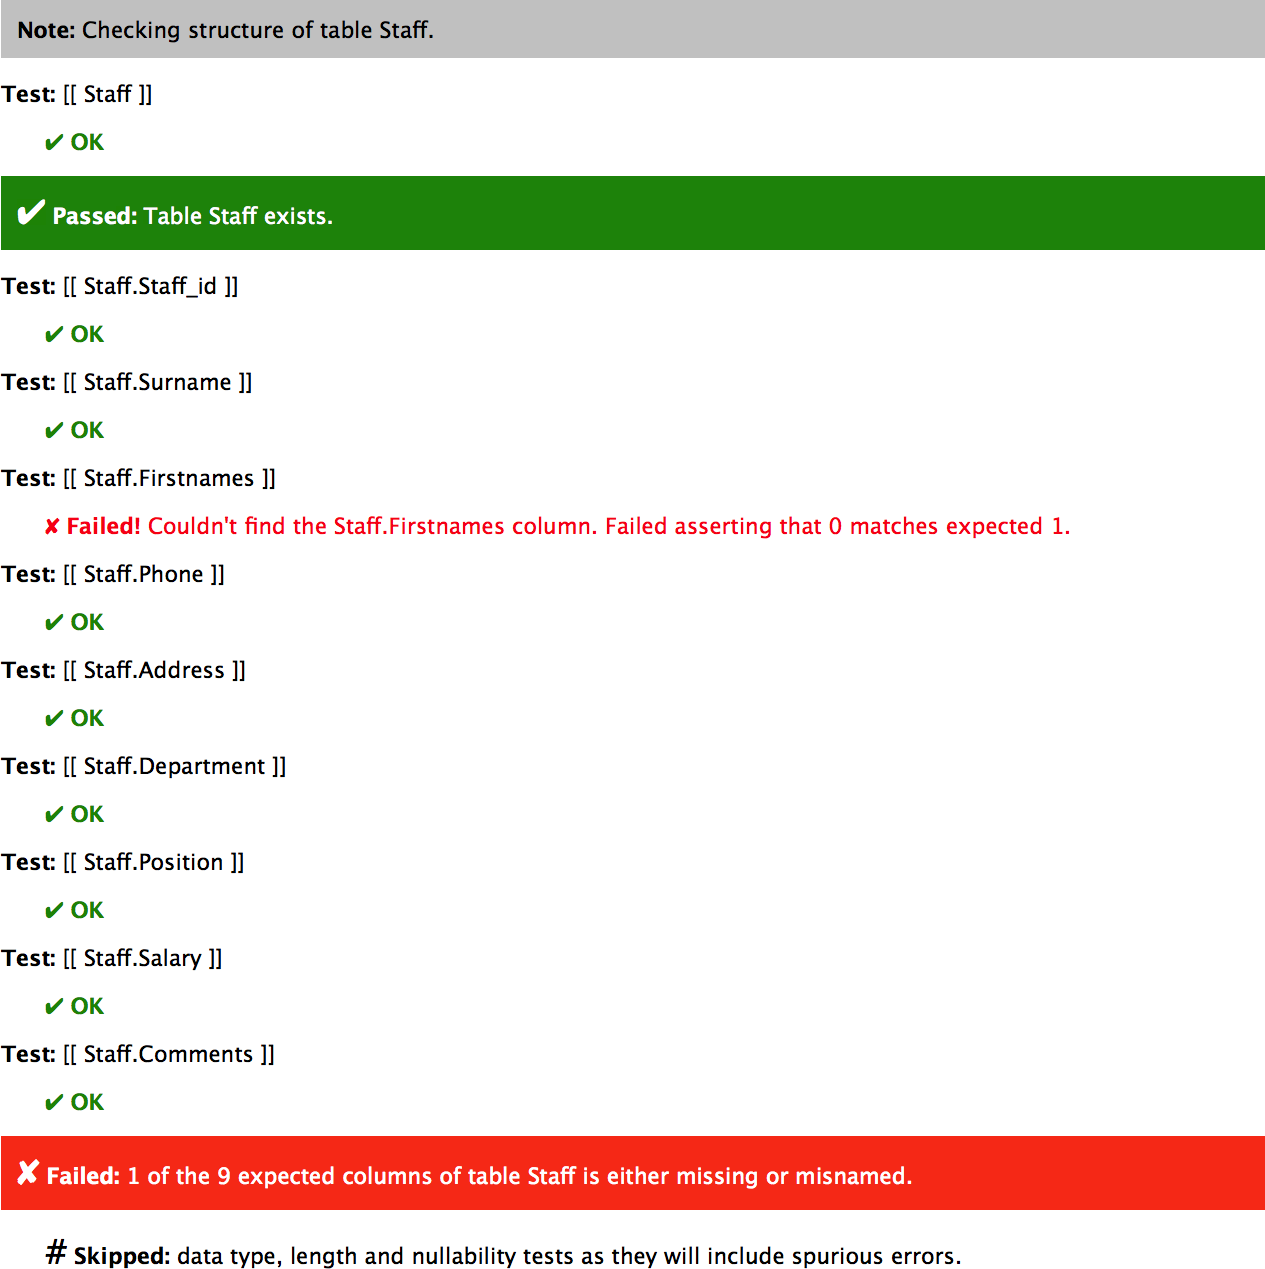
\includegraphics[width=0.95\columnwidth,keepaspectratio]{images/web_output.png}
    \caption{Example of web output}
\end{figure}


\begin{table}
    \footnotesize
%     \hrule
    \begin{verbatim}
public function getTableName()
{
    return 'PRODUCT';
}

public function getColumnList()
{
    return array(
        'PRODUCT_CODE' => array(
            'generic_type' => 'NUMBER',
            'sql_type' => array('NUMBER', 'INTEGER'),
            'min_length' => 8, 'max_length' => 8, 'decimals' => 0,
            'test_value' => 87654321, 'nullable' => false),
        'DESCRIPTION' => array( ... ),
        'STOCK_COUNT' => array(
            'generic_type' => 'NUMBER',
            'sql_type' => array('NUMBER', 'INTEGER'),
            'min_length' => 5, 'max_length' => 6, 'decimals' => 0,
            'underflow' => -1, 'overflow' => 100000,
            'legal_values' => array(0, 99999), 'test_value' => 456,
            'nullable' => false),
        'RESTOCK_LEVEL' => array( ... ),
        'MINIMUM_LEVEL' => array( ... ),
        'LIST_PRICE' => array(
            'generic_type' => 'NUMBER',
            'sql_type' => array('NUMBER', 'INTEGER'),
            'min_length' => 7, 'max_length' => 8, 'decimals' => 2,
            'underflow' => -0.01, 'overflow' => 100000.00,
            'legal_values' => array(0, 99999.99), 'test_value' => 123.99,
            'nullable' =>  false),
        'ASSEMBLY_MANUAL' => array(
            'generic_type' => 'BINARY',
            'sql_type' => array('BLOB'),
            'test_value'    =>  "NULL",
            'nullable' => true),
        'ASSEMBLY_PROGRAM' => array( ... )
    );

}

public function getPKColumnList()
{
    return array( 'PRODUCT_CODE' );
}

public function getFKColumnList()
{
    return array();
}   \end{verbatim}
%     \hrule
    \caption{Example of table specification}
\end{table}

\begin{figure}
    \sffamily
    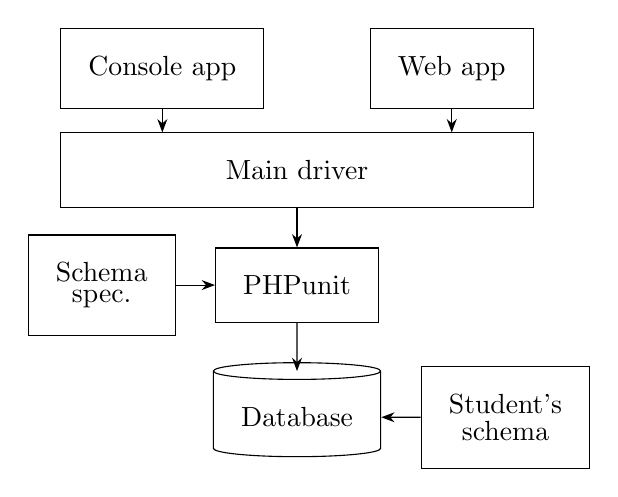
\begin{tikzpicture}[every node/.style={draw, minimum height=7.5mm, inner sep=1em}]
        \node (console) {Console app};
        \coordinate[below=3mm of console.south] (console port);
        
        \node[anchor=north west, minimum width=6cm] (driver) at ($(console.south west) - (0,3mm)$) {Main driver};
        
        \node[anchor=south east] (web) at ($(driver.north east) + (0,3mm)$) {Web app};
        \coordinate[below=3mm of web.south] (web port);
        
        \node[below=5mm of driver] (phpunit) {PHPunit};
        
        \node[left=5mm of phpunit] (spec) {\shortstack{Schema \\ spec.}};
        
        \node[cylinder, shape border rotate=90, below=5mm of phpunit, aspect=0.1] (database) {Database};
        
        \path (database.before top) -- (database.after top) coordinate[midway] (dbtop);
        
        \node[right=5mm of database] (schema) {\shortstack{Student's \\ schema}};
        
        \graph { [edges={draw, arrows={-{Stealth}}}]
            {(console), (web)} -> {(console port), (web port)},
            {(driver), (spec)} -> (phpunit),
            (phpunit) -> (dbtop),
            (schema) -> (database),
        };
    \end{tikzpicture}
    \caption{System architecture}
\end{figure}



\section{Evaluation}
\label{sec-evaluation}

\section{Conclusions \& future work}
\label{sec-conclusion}

\newpage\mbox{}\newpage
\bibliographystyle{ACM-Reference-Format}
\bibliography{Koli_2017_Stanger}

\end{document}
